\documentclass[11pt]{article}

\newcommand{\lectureNum}{02}
\newcommand{\lectureName}{Data Formats \& Encoding I}
\newcommand{\lectureDate}{2024-01-24}

\usepackage{../dbnotes}

\begin{document}

\maketitle
\thispagestyle{plain}

%% ==================================================================
%% INTRODUCTION
%% ==================================================================
\section{Introduction}

As the business landscape embraces data-driven approaches for analysis and decision-making, there is a rapid surge in the volume of data requiring storage and processing. This surge has led to the growing popularity of OLAP database systems, and the emergence of the lakehouse architecture has gained attention. The lakehouse architecture is designed to efficiently store vast amounts of data while concurrently offering robust data management capabilities, such as transaction handling. This lecture delves into the storage and representation of data within a DBMS, exploring how formats and encodings are tailored to align with the modern architecture of databases.

%% ==================================================================
%% Storage Model
%% ==================================================================
\section{Storage Model}

A DBMS's storage model specifies how it physically organizes tuples on disk and in memory.

%% ----------------------------------------------------
%% N-ary Storage Model (NSM)
%% ----------------------------------------------------

\subsection*{N-ary Storage Model (NSM)}

The DBMS stores (almost) \textbf{all attributes} for a single tuple contiguously in a single page for NSM. It's ideal for \textbf{OLTP} workloads because transactions tend to access individual entities and insert-heavy workloads. The page size is relatively small (e.g. 4KB) because it has to fit in the memory.

%% ----------------------------------------------------
%% Decomposition Storage Model (DSM)
%% ----------------------------------------------------
\subsection*{Decomposition Storage Model (DSM)}

The DBMS stores a single attribute for all tuples contiguously in a block of data for DSM \cite{10.1145/1376616.1376712}. It's ideal for OLAP workloads where file sizes are relatively large (e.g. 100MB) and read-only queries perform large scans over a subset of the table's attributes. Furthermore, for DSM, all variable length data needs to be converted to fixed length so that simple arithmetic can be used to jump to an offset to find a tuple. This can be done by using dictionary compression. The DBMS stores the dictionary in the header of the page and stores the actual data in the body of the page. The DBMS can then use the dictionary to reconstruct the data.

For tuple identifications of DSM, there are typically two choices:

\begin{itemize}
    \item \textbf{Fixed-length Offsets:} Each value is the same length for an attribute. The DBMS can reach locations of other attributes of the same tuple by inferring from the length of the value and the current offset.
    \item \textbf{Embedded Tuple Ids:} Each value is stored with its tuple ID in a column.
\end{itemize}

%% ----------------------------------------------------
%% Hybrid Storage Model (PAX)
%% ----------------------------------------------------
\subsection*{Hybrid Storage Model (PAX)}

Partition Attributes Across (PAX) is a hybrid storage model that vertically partitions attributes within a database page. It horizontally partitions data into row groups, and then vertically partitions their attributes into column chunks.

In most PAX models like Parquet \cite{zeng2023empirical} and ORC, the global metadata is at the bottom like \cref{fig:pax-file} because most distributed file systems are very append-friendly and may not support in-place updates efficiently. 

\begin{figure}[htbp]
    \centering
    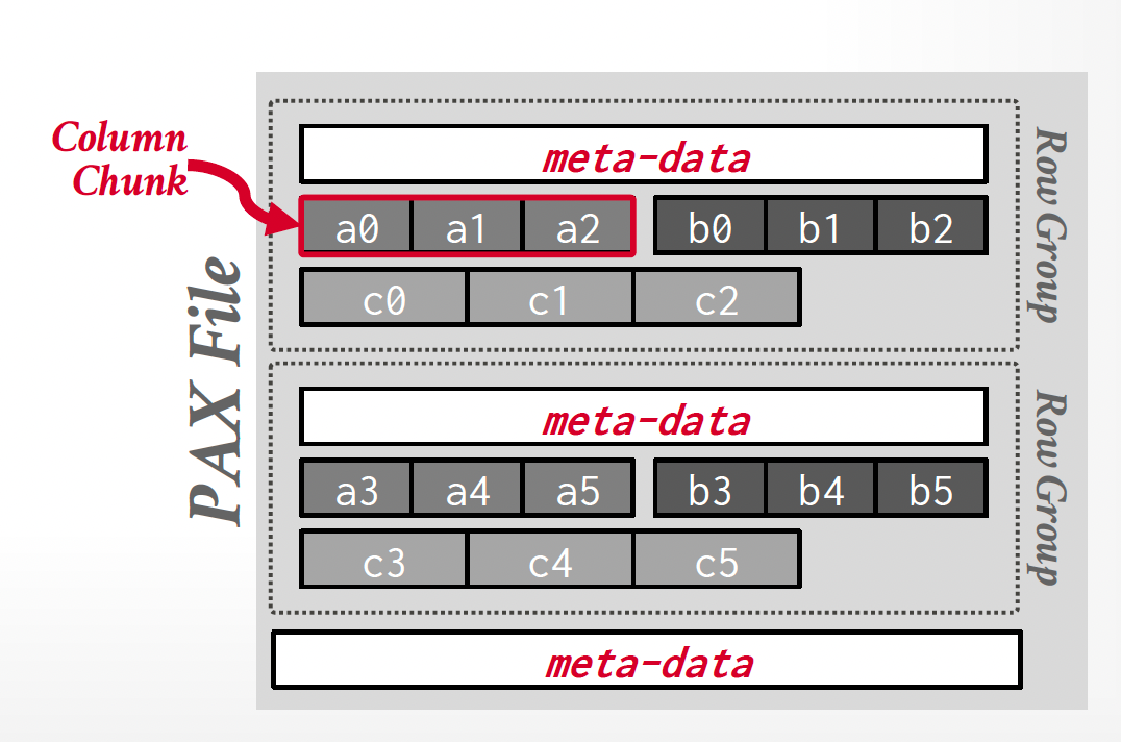
\includegraphics[width=0.7\textwidth]{fig/pax-file.pdf}
    \caption{PAX File Format}
    \label{fig:pax-file}
\end{figure}

%% ==================================================================
%% Format Design Decisions
%% ==================================================================
\section{Format Design Decisions}

All modern storage models (like Parquet and ORC) make certain design decisions.

%% ----------------------------------------------------
%% File Meta-data
%% ----------------------------------------------------
\subsection*{File Meta-Data}

Files are \textbf{self-contained} to increase portability. They contain all the necessary information to interpret their contents without external data dependencies. For example, the database pages contain all the information of the database and the tables. Also, all global metadata like table schema, row group offsets/length, tuple counts, and zone maps, must be serialized.

%% ----------------------------------------------------
%% Format Layout
%% ----------------------------------------------------
\subsection*{Format Layout}

The most common formats today use the PAX storage model. For example, the size of the row group varies per implementation and makes compute-memory trade-offs. The determination criteria of the row group in the prevalent formats today are as follows:

\begin{itemize}
    \item Parquet: Number of tuples (e.g. 1 million)
    \item ORC: Physical storage size (e.g. 250 MB)
    \item Arrow: Number of tuples (e.g., 1024 *1024)
\end{itemize}

%% ----------------------------------------------------
%% Type System
%% ----------------------------------------------------
\subsection*{Type System}

The type system defines the data types that the format supports. A database system typically has both physical types and logical types:

\begin{itemize}
    \item \textbf{Physical Type}: Low-level byte representation (e.g. IEEE-754).
    \item \textbf{Logical Type}: Auxiliary types that map to physical types. As an illustration, contemporary storage models typically use an INT64 type value to store timestamps, representing the count of seconds or milliseconds that have elapsed since the epoch.
\end{itemize}

%% ----------------------------------------------------
%% Encoding Schemes
%% ----------------------------------------------------
\subsection*{Encoding Schemes}

Encoding schemes specify how the format stores the bytes for contiguous/related data. Several encoding schemes can be applied on top of each other to further improve compression.

One type of encoding scheme is \textbf{dictionary encoding}. It replaces frequent values with smaller fixed-length codes and then maintains a mapping (dictionary) from the codes to the original values.

\begin{figure}[htbp]
    \centering
    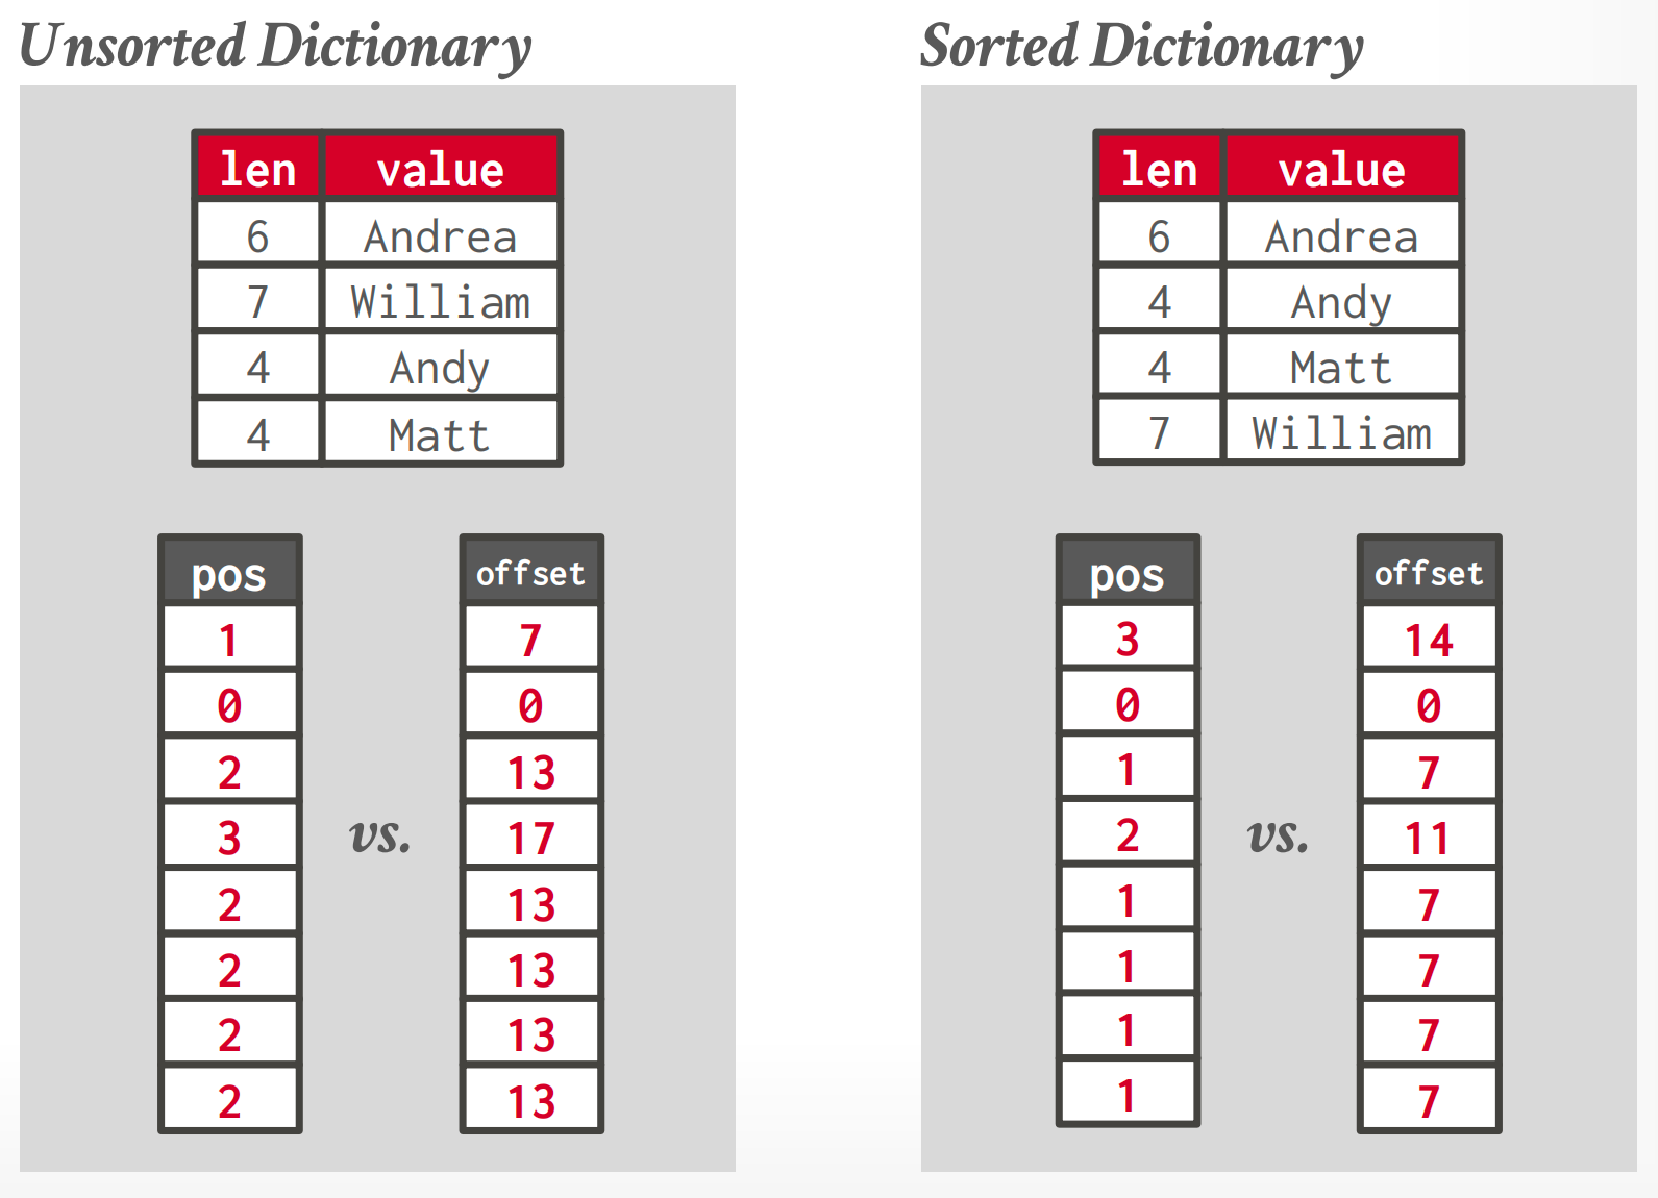
\includegraphics[width=0.7\textwidth]{fig/dict-encoding.pdf}
    \caption{Dictionary Encoding}
\end{figure}

File formats must handle the case where the number of distinct values (NDV) in a column chunk is too large. Here is what Parquet and ORC do:
\begin{itemize}
    \item \textbf{Parquet}: Limit the max dictionary size as 1MB.
    \item \textbf{ORC}: Pre-compute the NDV and disable dictionary encoding if it is too large.
\end{itemize}

There are other encoding schemes like run-length encoding (RLE), bit packing, delta encoding, and frame-of-reference (FOR), which are widely used in real-world systems.

%% ----------------------------------------------------
%% Block Compression
%% ----------------------------------------------------
\subsection*{Block Compression}

Block compression compresses data using a general-purpose algorithm (e.g. Zstd). It saves the storage space, but can introduce computation overhead and data opacity for the execution engine. Block compression was useful years ago when networks and disks were slow and it was expensive to retrieve data from the disk and send it over the network. Today, however, we have cheap object stores, so block compression has become less helpful.

%% ----------------------------------------------------
%% Filters
%% ----------------------------------------------------
\subsection*{Filters}

There are several types of filters in database systems to boost the searching performance:

\begin{itemize}
    \item \textbf{Zone Maps}: Maintain min/max values per column at file level and row group level. It is more effective if values are clustered.
    \item \textbf{Bloom Filters}: Rack the existence of values for each column in a row group. There can be a false positive for a bloom filter, where the value actually does not exist in the storage.
\end{itemize}

%% ==================================================================
%% Nested Data
%% ==================================================================
\section{Nested Data}
In order to store real-world semi-structured data as regular columns, most modern formats add additional fields that make querying the data easier and faster. 

%% ----------------------------------------------------
%% Nested Data: Shredding
%% ----------------------------------------------------
\subsection*{Nested Data: Shredding}
In the Nested Data Shredding approach, the following two additional fields are stored:

\begin{itemize}
    \item \textbf{Repetition Level}: At what repeated field in the field's path the value has repeated.
    \item \textbf{Definition Level}: Specifies how many columns in the path of the field that could be undefined are actually present \cite{Dremel}.
\end{itemize}

\begin{figure}[htbp]
    \centering
    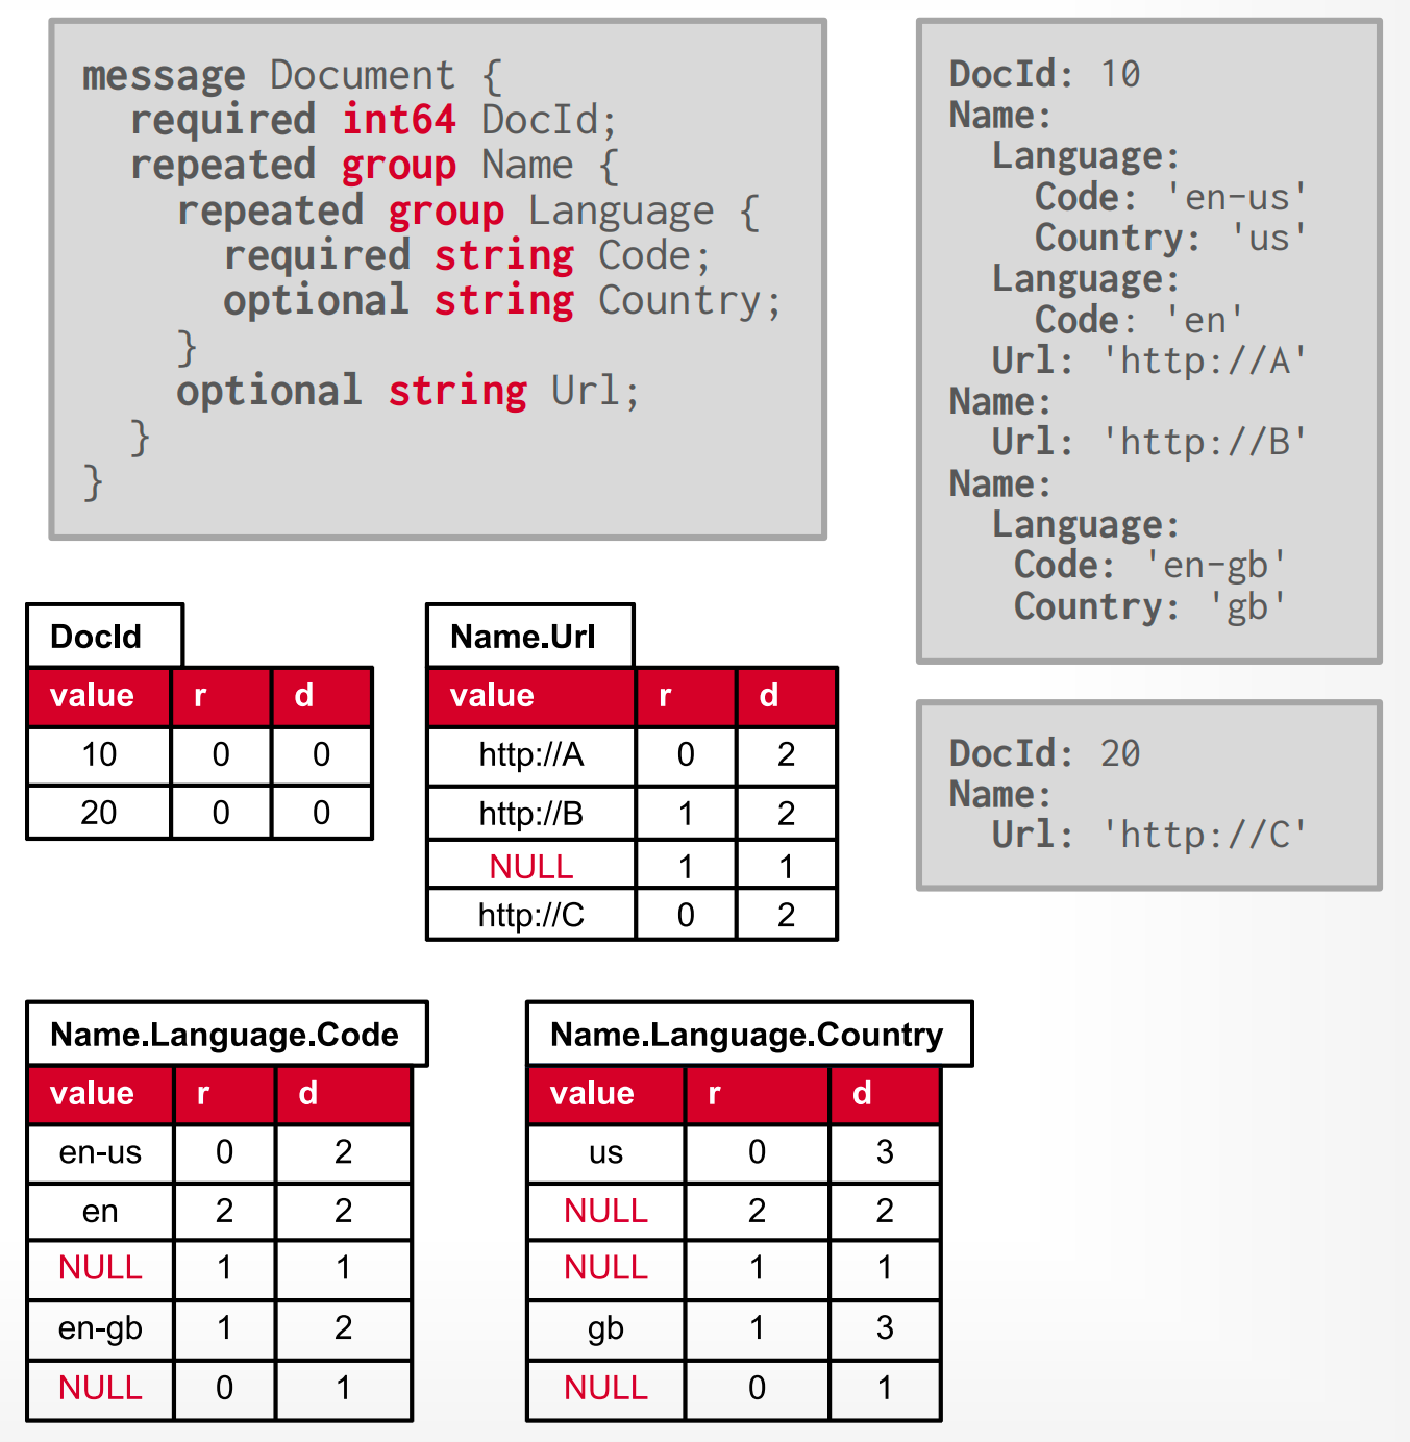
\includegraphics[width=0.7\textwidth]{fig/nested-data-encoding.pdf}
    \caption{Shredding Encoding for Nested Data}
\end{figure}


%% ----------------------------------------------------
%% Nested Data: Length + Presence
%% ----------------------------------------------------
\subsection*{Nested Data: Length + Presence}
Another way to store nested structures as separate columns is to track the number of entries at each path level (\textbf{length}) and whether a key exists at that level for a record (\textbf{presence}).

%% ==================================================================
%% Lessons from the Real World
%% ==================================================================
\section{Lessons from The Real-World}
Analysis of synthetic real-world data sets in \cite{zeng2023empirical} on Arrow's C++ Parquet/ORC libraries presents certain key insights. Here are the key takeways:
\begin{itemize}
    \item Due to the repetitiveness of data in the real world, dictionary encoding is a viable option for all data types and not just strings.
    \item Simplistic encoding schemes can be decoded much faster due to a decrease in branch mispredictions at runtime.
    \item Block compression is becoming unnecessary as network and disk are becoming faster and CPU is becoming the bottleneck.
\end{itemize}



% ==================================================================
% BIBLIOGRAPHY
% ==================================================================
\newpage
\bibliographystyle{abbrvnat}
\bibliography{02-data1}

\end{document}
